\section{Extension du support exécutif}\label{sec:openmp:runtime}

Cette partie complète la section précédente, puisqu'elle se concentre sur l'exploitation des informations fournies par l'utilisateur, ainsi que sur la prise en compte des architectures NUMA côté support exécutif.

Ces extensions ciblent des supports exécutifs fonctionnant par vol de travail (voir section~\ref{sec:context:runtimes:ws}), et ont été implémenté dans Kaapi ainsi que libKOMP (TODO: ref aux sections décrivant ça ?).

\subsection{Hiérarchiser le support exécutif}

La modification la plus importante consiste à hiérarchiser les files de tâches pour le vol de travail, puisque c'est là dessus que ce base l'ordonnancement.

Des outils tels que hwloc permettent de donner des informations sur la hiérarchie, nous avons donc des informations précises sur quel cœur est placé physiquement sur quel nœud NUMA, et nous avons donc pu mettre en place une hiérarchie dans les files de tâches :

\begin{itemize}
  \item Chaque cœur possèdent deux files de tâches : une publique, dans laquelle les autres cœurs peuvent venir voler ; et une privée, dans laquelle tout le monde peut venir ajouter des tâches, mais seul le cœur propriétaire peut venir voler.
  \item Chaque nœud possèdent également deux files de tâches, suivant le même principe que précédemment. Pour la file privée, seuls les cœurs situés sur le nœud NUMA propriétaire peuvent venir voler des tâches.
\end{itemize}

Nous avons également fait en sorte d'allouer la mémoire manipulée par les différentes files sur le nœud NUMA sur lequel cette file est située.



\subsection{Heuristiques basées sur la localité des données}\label{sec:contrib:ws:heuristics}

Comme décrit dans la section~\ref{sec:context:runtimes:ws}, le vol de travail repose sur deux étapes essentielles : la sélection d'une file de tâches lors du vol, et le choix d'une file lorsqu'une tâche devient prête.

Les deux sections suivantes décrivent les modifications que nous avons mis en place dans le support exécutif, dans l'objectif de prendre en compte le côté NUMA de l'architecture.
Ces travaux ont été publiés à EuroPar 2016~\cite{Virouleau2016b}.


\subsubsection{Distribution des tâches prêtes : stratégies de \emph{placement}}
\label{sec:openmp:runtime:push}

Nous introduisons quatre stratégies différentes pour le placement des tâches prêtes, vis à vis des files de tâches hiérarchiques définies dans la section précédente.
Deux d'entre elles sont indépendantes des données, alors que les deux autres prennent en compte les informations fournies par l'utilisateur via la clause |affinity| décrite dans la section~\ref{sec:openmp:langage:affinity}, ou à défaut utilisent des informations issues des dépendances de données.

\begin{description}
  \item [pLoc :] le processeur responsable du placement de la tâche place celle ci dans sa propre file - \emph{\textbf{p}lacement\textbf{Loc}al}.
  \item [pLocNum :] la stratégie agie de manière similaire à la précédente, à ceci près que le processeur place celle ci dans la file de son nœud NUMA - \emph{\textbf{p}lacement\textbf{Loc}al\textbf{Num}a}.
  \item [pNumaW :] le processeur responsable du placement de la tâche regarde si une affinité de donnée est spécifiée, si aucune affinité n'est présente, il utilise une des dépendances en écriture de la tâche comme affinité.
Il détermine ensuite le nœud NUMA sur lequel a été allouée la donnée, et place la tâche dans la file du nœud correspondant.
  \item [pNumaWLoc :] la stratégie agie de manière similaire à la précédente, mais si le nœud NUMA déterminé correspond au nœud NUMA du processeur courant, alors la tâche est poussée dans la file du processeur directement.
\end{description}

Un détail distingue les deux premières stratégies des deuxx secondes : dans le cas des stratégies |pLoc| et |pLocNum|, le placement initial des données n'est pas pris en compte, alors que les stratégies |pNumaW| et |pNumaWLoc| utilisent toutes deux les informations sur l'allocation physiques des données manipulées par la tâche.

\subsubsection{Équilibrage de charge dynamique : stratégie de \emph{sélection}}
\label{sec:openmp:runtime:select}


Nous avons implémenté un ensemble de stratégie de sélection de files de tâches, qui ont conscience de la topologie de l'architecture sur laquelle est exécutée le programme.

Les deux premières sont similaires aux travaux effectués par Olivier et al.~\cite{Olivier2012} :
\begin{description}
  \item [sRand :] sélection aléatoire d'une file parmi les files des cœurs.
  \item [sRandNuma :] sélection aléatoire d'une file parmi les files des nœuds.
\end{description}

Ces deux stratégies pourront servir de base de comparaison avec les stratégies suivantes, prenant en compte les deux niveaux de hiérarchie disponibles, ainsi que la notion de << voisinage >> entre cœurs.

\begin{figure}[t!]
  \centering
  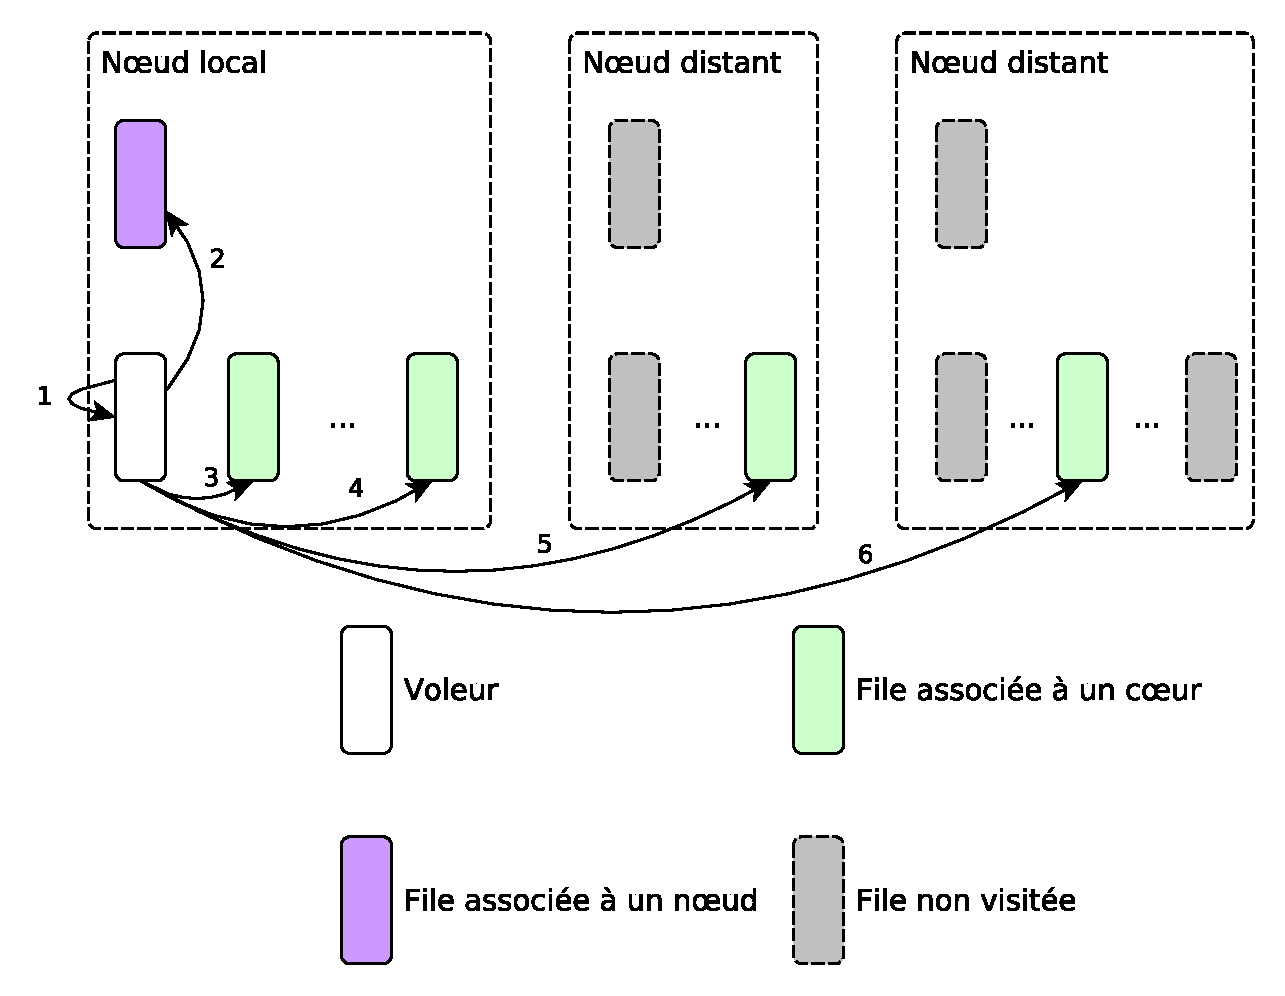
\includegraphics[width=0.73\textwidth]{steal_strategies_proc}
  \caption{Illustration de la stratégie \emph{sProc}, avec l'ordre de visite des files}\label{fig:openmp:runtime:steal_proc}
\end{figure}

\begin{figure}[h!]
  \centering
  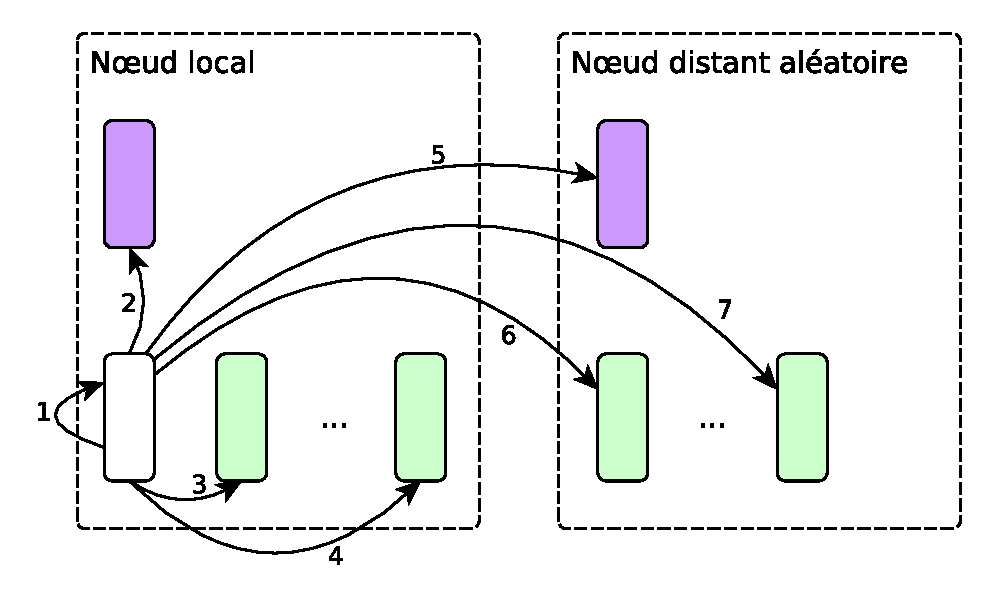
\includegraphics[width=0.6\textwidth]{steal_strategies_numa_proc}
  \caption{Illustration de la stratégie \emph{sNumaProc}, avec l'ordre de visite des files}\label{fig:openmp:runtime:steal_numa_proc}
\end{figure}

\begin{description}
  \item [sProc :] Cette stratégie est illustrée sur la figure~\ref{fig:openmp:runtime:steal_proc}. Le voleur va visiter sa propre file (1), celle de son nœud NUMA (2), puis va parcourir uniquement les files des cœurs en commençant par ses voisins (3, 4), puis en choisissant au hasard parmi les cœurs distant restant (5, 6).
  \item [sNuma :] Le voleur commence par visiter son nœud NUMA, puis les files des cœurs de son nœud, puis uniquement les files des nœuds NUMA distant.
  \item [sProcNuma :] Dans un premier temps le cœur voleur visite sa propre file. Si aucune tâche n'est disponible, il va ensuite visiter les files de tâches des cœurs voisins situés sur le même nœud.
    Si cela échoue de nouveau, il ira voler la file de son nœud NUMA.
    Si cela également, le reste de la topologie sera parcourue de manière similaire : un nœud sera choisi aléatoirement, les files des cœurs puis celle du nœud seront visitées.
  \item [sNumaProc :] Cette stratégie est illustrée sur la figure~\ref{fig:openmp:runtime:steal_numa_proc}~; elle est similaire à la précédente, mais l'ordre de parcours est inversé : après avoir visité sa propre file (1) le voleur regarde d'abord les files des nœuds NUMA (2) avant de regarder les files des cœurs (3, 4). De même que pour la stratégie précédente, le reste de la topologie est parcourue de manière similaire (5, 6, 7).
\end{description}


\subsection{Distribution des tâches d'initialisation}


La section~\ref{sec:openmp:langage:init} décrit comment un utilisateur peut avoir du contrôle sur la distribution des données de son application.
Cela passe par la distribution des tâches d'initialisation, et nécessite donc une modification du support exécutif.

Nous avons implémentés des stratégies additionnelles de placement des tâches prêtes, qui sont prioritaires sur toute autre stratégie décrite dans la section précédent, si une clause |init| est présente.
Elles correspondent directement aux stratégies décrites dans la section~\ref{sec:openmp:langage:init} : \textbf{random}, \textbf{cyclic}, \textbf{cyclicnuma}, et ont naturellement été implémentée en utilisant les files correspondantes de la hiérarchie.

\begin{todo}
  L'intérêt ici était de distinguer ce qu'on propose comme choix à l'utilisateur et comment c'est implémenté derrière.
  Mais bon ça fait un peu maigre comme section...
\end{todo}


\subsection*{Conclusion}

L'ensemble de ces modifications proposent un large choix de paramètres à ajuster pour le support exécutif, et ce n'est pas évident de voir a priori quelle(s) stratégie(s) devraient être privilégiée(s).

Y en a-t-il des meilleures que d'autres quelques soient les circonstances ?
Est-ce que que cela dépend du type d'application ? Du type d'architecture ?
La section suivante propose une évaluation détaillée de l'impact des différents points, et vise à dégager des conseils généraux vis à vis du choix des stratégies.

